\documentclass[12pt]{article}

\usepackage{color,graphicx,overpic}
\usepackage[margin=1.0in]{geometry}

\begin{document}
\noindent\textsc{\large CS 314 Final Review --- Reverse Doubly Linked List --- \textbf{Solution}}

\vspace{6pt}
\noindent\textbf{Linked Lists}

\vspace{2pt}
\noindent  Write an instance method for a doubly linked list which reverses the order of the elements in the list. The first element will 
become the last element, the second becomes the second-to-last, etc. 

\vspace{4pt}
\noindent The doubly linked list class provided, \texttt{DoubleLinkedList}, has doubly linked nodes and the list is null terminated at both ends.
There are no special header nodes, all nodes contain elements of the list. The list object holds references to the first
and last elements in the list. The following is a visual digram of this list class:

% List diagram
\begin{figure}[h!]
  \hfill
  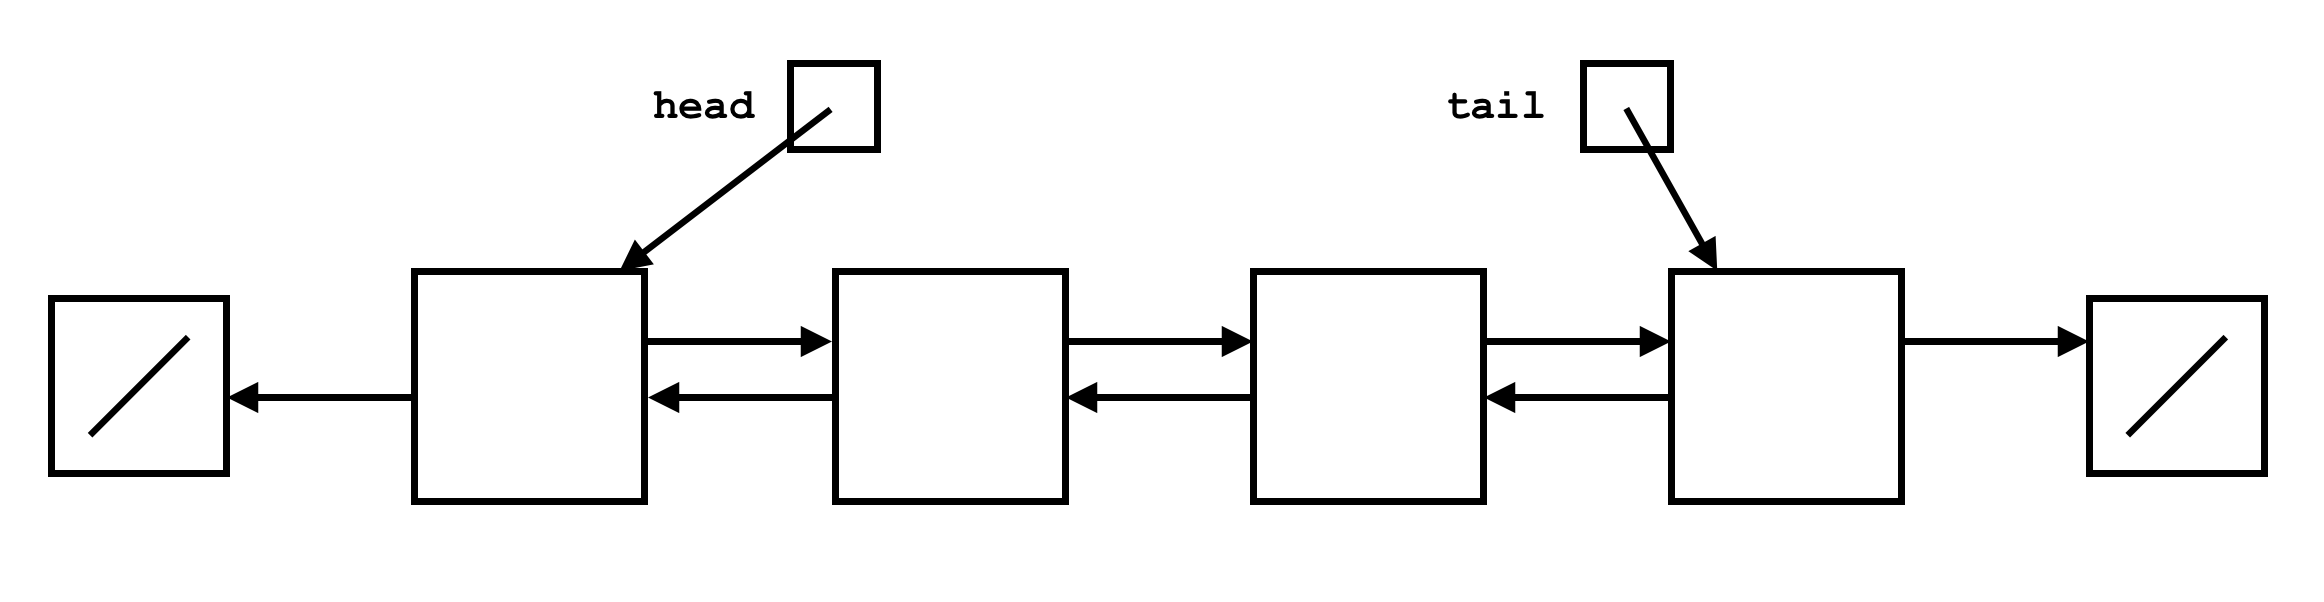
\includegraphics[width=115mm, scale=0.5]{diagram.png}
  \hspace*{\fill}
\end{figure}

\noindent Examples of calls to \texttt{reverseList()}. The result shown is the new state of \texttt{this}.
\begin{itemize}
  \item \texttt{[0, 1, 2, 3].reverseList() => [3, 2, 1, 0]}
  \item \texttt{[3, 1, 4].reverseList() => [4, 1, 3]}
  \item \texttt{[5, 5, 5].reverseList() => [5, 5, 5]}
  \item \texttt{[7].reverseList => [7]}
  \item \texttt{[].reverseList => []}
\end{itemize}

\vspace{6pt}
\noindent Use the follwing \texttt{DoubleLinkedList} implementation.
\begin{verbatim}
public class DoubleLinkedList<E>{

    private DoubleListNode<E> head, tail;
    private int size;
   
    // Inner node class 
    private static class DoubleListNode<E>{
      DoubleListNode<E> prev, next;
      E data;
    }
}
\end{verbatim}

\noindent \textbf{You may not create any new data structures.}

\noindent No methods are provided. Do not use any other Java classes.

\clearpage
\begin{verbatim}
/* 
 * Pre:  none
 * Post: oldSize == newSize, 'this' list is reversed
 */
public void reverseList(){
    DoubleNode<E> currNode = head;

    while(currNode != null){
        //Swap this node's next and prev references
        DoubleNode<E> temp = currNode.next;
        currNode.next = currNode.prev;
        currNode.prev = temp;

        //The next node is now the prev node because of swap
        currNode = currNode.prev;
    }

    //Swap the head and tail references
    DoubleNode<E> oldHead = head;
    head = tail;
    tail = oldHead;
}
\end{verbatim}
\end{document}
